\begin{figure}[htb!]
    \centering
    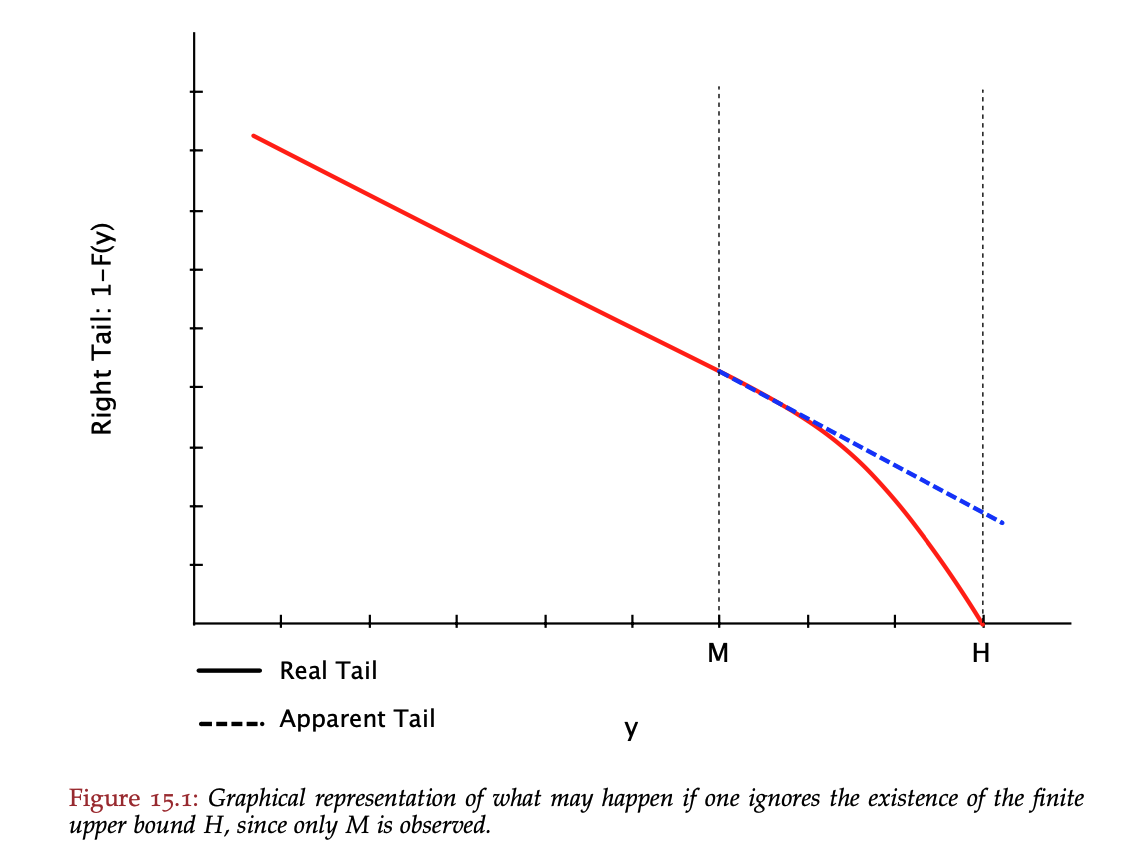
\includegraphics[width=1\linewidth]{images/nnt-upper-bound.png}
    \vspace{-15pt}
   \caption{As shown in this Figure from T19~\cite{taleb2019statistical} if you only
   observe a distribution up to some value M, you may be tempted to fit a line through the
   data (dotted blue line). But if there were in fact a limit to the distribution at H,
   you would be overestimating the true number of very extreme events (red curve)
   and also predict events that were larger than were possible.  }
   \label{fig:up-bound-taleb}

\end{figure}
